\documentclass[12pt, letterpaper]{article}
\usepackage[utf8]{inputenc}
\usepackage[margin=1in]{geometry}
\usepackage{graphicx}
\usepackage{amsmath}
\usepackage{indentfirst}

\setlength{\parskip}{1em}


\title{Modelling Carbon Content in Soil Pools with Stochastic Rainfall on the Island of Hawai'i}
\author{Kat Contreras-Godfried \\ CEE '22 \and 
        Katie Irelan \\ EEB '22 \and 
        Connor Larson \\ ORF '22}
\date{May 10, 2021}

\begin{document}

\maketitle

\begin{center}
    
\includegraphics[width=0.15\textwidth]{shield.png}
\end{center}


\begin{abstract}
    This model couples a stochastic soil moisture model to the soil carbon cycle, represented by three differential equations based on a previous model. Soil moisture and carbon are linked to one another in this model through hydrological controls on the rate of microbial decomposition. We then applied the model to a precipitation gradient on a volcano on the island of Hawai’i, Mauna Kea, in order to show alterations in carbon cycle as a result of moisture changes on short- and long-term bases.
\end{abstract}

\section{Introduction}

In this model, we linked a soil moisture model based on stochastic rainfall to the soil carbon cycle, represented by three differential equations for each pool of carbon. The goal of this model is to explore and work to predict the relationship between water and nutrient cycling in soil systems. Empirically, alterations in soil moisture have been shown to cause changes in soil nutrient availability and cycling. \cite{kramer_controls_2016,schimel_life_2018} This is important to understand in order to predict how ecosystems may respond to the increasing frequency of water-related climate crises. \cite{oconnell_drought_2018}

We drew heavily on an existing model by Porporato et. al, which depicted the hydrological controls on both the carbon and nitrogen cycles. \cite{porporato_hydrologic_2003} After building the model, we applied it to Mauna Kea, a volcano in Hawai’i that has pronounced changes in rainfall with elevation. \cite{bateman_quantitative_2019} Hawaii has many ecological gradients that have been used to ask questions about ecosystem responses to changing resources. In our application, we used parameters based on three areas along the gradient with differing rainfall levels to show how carbon availability is altered both on a short-term basis with individual rainfall events and with long-term differences in precipitation patterns. 

\section{Methodology}
\subsection{Rainfall}

Rainfall is simulated via a stochastic process drawn from two distributions. First, rainfall events are modelled as a Poisson process with rate $\lambda = \frac{RainyDays}{365}$ - intuitively, the probability of any day being “rainy.” In our discrete-time model, this is generated via a binomial approximation with probability of any time-step being rainy being:

$$ P(Rainy) = P(U < \Delta t \lambda) $$

Here, $U$ is a uniformly drawn random variable on $[0,1)$ and $\Delta t$ is in units ${days}^{-1}$. Next, rainfall amounts are drawn for each event from an exponential distribution with mean $\mu = \frac{YearlyRainfall}{RainyDays}$. These are generated via the inverse CDF:

$$ h = -\mu \ln{U} $$

Thus, a time-series $\hat{h}$ is generated with each time step having value $0$ or a rainfall amount $h$.

\subsection{Soil Moisture}

Using the time-series of rainfall as input, changes in soil moisture are calculated via forward-Euler as the sum of gains from Infiltration and losses from Evaporation, Transpiration, and Leakage:

$$ n Z \Delta s = I(s, h) - \Delta t \left[ E(s) + T(s) + L(s) \right]$$

Above, $n$ is the soil porosity and $Z$ is the soil depth.

Infiltration is, in most cases, simply the magnitude of rainfall per area, as simulated in the previous step. However, because total soil moisture cannot exceed 1, it is limited by the remaining capacity of the soil:

$$ I(s, h) = \min{[h, n Z (1-s)]} $$

Evaporation is a non-linear function of soil moisture: below the hygroscopic point $s_h$, water does not evaporate; between this and the wilting point $s_w$, evaporation linearly increases to a maximum value $E_{max}$; and, above the wilting point, evaporation is constant.

$$ E(s) = \begin{cases}
			0 & \text{if $s < s_h$}\\
            \frac{s - s_h}{s_w - s_h} E_{max} & \text{if $  s_h < s < s_w $}\\
            E_{max} &  \text{if $s > s_w $}
		 \end{cases} $$
		 
Transpiration is a similar non-linear function of soil moisture: below the wilting point, there is no transpiration; above the wilting point but below the water stress point $s^*$, transpiration increases linearly to a maximum value $T_{max}$; and, above the wilting point, transpiration is constant. 

$$ T(s) = \begin{cases}
			0 & \text{if $s < s_w$}\\
            \frac{s - s_w}{s_w - s^*} T_{max} & \text{if $  s_w < s < s^* $}\\
            T_{max} &  \text{if $s > s_* $}
		 \end{cases} $$

Finally, leakage is a nonlinear function of soil moisture dependent on the saturated hydraulic conductivity of the soil $K_s$, a constant $\beta = 2b+4$ dependent on the soil porosity index $b$, and the soil field capacity $s_{fc}$.

$$ L(s) = \begin{cases}
			0 & \text{if $s < s_fc$}\\
            K_s \frac{e^{beta (s - s_{fc})} - 1}{e^{beta (1 - s_{fc})} - 1} &  \text{if $s > s_fc $}
		 \end{cases} $$



With these equations and the forward-Euler method, given an initial value $s_0$, a time-series can be iteratively produced for soil moisture using the simulated rainfall data.


\subsection{Carbon Cycle}
Finally, given a time-series of soil moisture data, a box model can be used to approximate the carbon cycle in the three pools: litter, humus, and biomass. The carbon cycle is linked to soil moisture via a decomposition function:

$$ f_d(s) = \begin{cases}
			\frac{s}{s_{fc}} & \text{if $s < s_fc$}\\
            \frac{s_{fc}}{s} &  \text{if $s > s_fc $}
		    \end{cases} $$

Decomposition in the litter pool is a function of this value, biomass carbon $C_b$, litter carbon $C_l$, and a rate parameter $k_l$:

$$ DEC_l = f_d(s) k_l C_b C_l $$

Similarly, decomposition in the humus pool is a function of the soil moisture, biomass carbon, humus carbon $C_h$, and a rate parameter $k_h$:

$$ DEC_h = f_d(s) k_h C_b C_h $$

Biomass death also contributes to the rate of carbon return to the litter pool, and is a linear function of biomass carbon proportional to a rate parameter $k_d$:

$$ BD = k_d C_b $$

Given these decomposition functions, the change in carbon content in each box is again calculated using forward-Euler. In the litter pool, carbon enters through litterfall $ADD$ and biomass microbial death, and leaves via decomposition:

$$ \frac{\Delta C_l}{\Delta t} =  ADD + BD - DEC_l  $$

In the humus pool, carbon enters as a fraction of the litter decomposition (proportional to the "isohumic coefficient" $r_h$ and leaves through humus decomposition:

$$ \frac{\Delta C_h}{\Delta t} = r_h DEC_l - DEC_h $$

Finally, carbon enters the biomass pool via litter decomposition (less the fraction that enters the humus and a fraction $r_r$ which goes to respiration) and humic decomposition (again less respiration), and leaves via microbial death $BD$:

$$ \frac{\Delta C_b}{\Delta t} = (1-r_h-r_r)DEC_l + (1-r_r)DEC_h - BD $$

With these equations, a time-series of soil moisture values, and a set of initial values $(C_{l0}, C_{h0}, C_{b0})$, the forward-Euler method can be used to calculate incremental changes and thus a time-series of carbon contents in each pool.

\section{Parameters}

To run the model, we constructed three sets of parameters for each rainfall level on Mauna Kea. On this volcano, rainfall levels relate inversely to elevation, meaning that lower elevations experience around 3500mm/year of rainfall while the highest elevations have extremely low levels of rainfall, around 500mm/year. At this high elevation level, vascular plants are not able to grow. Before that threshold, however, there are different ecosystems corresponding to moisture levels along the gradient. The wettest area is dominated by bogs and forest, followed by scrub forest dominated by \textit{M. polymorpha}, a shrub endemic to Hawaii, ultimately ending with savannah. In a study that measured environmental thresholds of soil fertility using the Mauna Kea gradient, soil nutrient content was measured at various points on the volcano. Using their measurements in combination with a study of how \textit{M. polymorpha} litterfall changes with rainfall, we were able to estimate different parameters to reflect these three areas as accurately as possible without collecting our own field data. \cite{bateman_quantitative_2019}

Apart from carbon content, litterfall, and rainfall changes, specific soil and vegetation parameters were difficult to find. For any remaining parameters, we used similar values to the companion paper to Porporato et. al, which applied that model to an African savanna ecosystem. \cite{dodorico_hydrologic_2003}


\begin{table}[p]
\begin{center}
\begin{tabular}{ c c c l }
Parameter & Value & Units & Description \\
\hline 
Days & 7300 & days & Number of days to run the model \\
Steps per day & 24 & - & Number of iterations per day \\
Rainy days &  73 & days & Average number of rainy days per year \\
Yearly rainfall & See below & mm/year & Average yearly rainfall \\
$Z$ & 300 & mm & Depth of soil layer \\
$n$ & 0.5 & - & Soil porosity \\
$s_h$ & 0.02 & - & Hygroscopic point \\
$s_w$ & 0.065 & - & Wilting point \\
$s^*$ & 0.17 & - & Water stress point \\
$s_{fc}$ & 0.3 & - & Field capacity \\
$E_{max}$ & See below & mm/day & Max evaporation \\
$T_{max}$ & See below & mm/day & Max transpiration \\
$b$ & 0.2 & - & Soil porosity index \\
$K_s$ & 1.1 & mm/day & Saturated hydraulic conductivity \\
$s_{init}$ & 0.11 & - & Initial soil moisture \\
$ ADD $ & See below & gC/(day*m\textsuperscript{2}) & Litterfall \\
$k_d$ & 8.5e-3 & 1/day & Biomass death rate parameter \\
$k_l$ & 6.5e-5 & m\textsuperscript{2}/(gC*day) & Litter decomposition rate parameter \\
$k_h$ & 2.5e-6 & m\textsuperscript{2}/(gC*day) & Humus decomposition rate parameter \\
$r_h$ & 0.25 & - & Isohumic coefficient \\
$r_r$ & 0.6 & - & Respiration coefficient \\
$C_{h,init}$ & See below & gC/m\textsuperscript{2} & Initial humus carbon \\
$C_{b,init}$ & See below & gC/m\textsuperscript{2} & Initial biomass carbon \\
$C_{l,init}$ & See below & gC/m\textsuperscript{2} & Initial litter carbon 

\end{tabular}
\end{center}
\caption{\label{tab:table-name}Model Parameters and Descriptions}
\end{table}

\begin{table}[p]
\begin{center}
\begin{tabular}{ c c c c c }
Parameter & 1500m & 2500m & 3500m & Unit \\
\hline 
Yearly rainfall & 3500 & 1200 & 500 & mm/year \\
$E_{max}$ & 0.8 & 0.9 & 1.0 & mm/day \\
$T_{max}$ & 3.3 & 3.7 & 4.0 & mm/day \\
$ADD$ & 0.5 & 0.6 & 0.7 & gC/(day*m\textsuperscript{2}) \\
$C_{h,init}$ & 7975 & 7000 & 13700 & gC/m\textsuperscript{2} \\
$C_{b,init}$ & 19 & 24 & 27 & gC/m\textsuperscript{2} \\
$C_{l,init}$ & 1240 & 1100 & 2160 & gC/m\textsuperscript{2} 

\end{tabular}
\end{center}
\caption{\label{tab:table-name}Altitude-dependent Parameter Values}
\end{table}

\emph{Rainfall Parameters}

We created a stochastic rainfall pattern based on how much rainfall there is on average in each of three areas per year and how many rainy days Mauna Kea experiences per year on average, which is 72. \cite{bateman_quantitative_2019,giambelluca_online_2013}

\emph{Soil Parameters}

These values usually need to be measured by taking soil samples and measuring weight, bulk density, saturation point, and other traits. However, these values tend to be linked to soil type and can therefore be estimated in that manner. Given that we are not able to take field measurements, we used a porosity value that reflects the average porosity of silty clay loam, which is the soil type most common in the Mauna Kea area. \cite{hato_soil_1973} In the study of soil thresholds on the volcano, the soil in each area of the gradient is categorized more specifically. \cite{bateman_quantitative_2019} However, any porosity values we chose would merely be estimated, so we used the same value for all three runs to reduce the chances of influencing our results incorrectly. 

Soil depth refers to the area of soil in which roots are able to extend. This model is only focused on how soil moisture and carbon change and are influenced by one another in relation to vegetation responses, meaning that including any dynamics below the root systems would unnecessarily complicate this model. We chose the value for this parameter based on the depth of soil measurements taken in the Mauna Kea soil study. \cite{bateman_quantitative_2019}

For the other soil parameters (field capacity and hygroscopic point), we used the values from the companion paper to Porporato et. al. \cite{dodorico_hydrologic_2003} These values would have to be measured through field tests and are difficult to approximate from other soil information.


\emph{Vegetation Parameters}

We scaled maximum evapotranspiration based on the aforementioned study of soil thresholds on Mauna Kea. \cite{bateman_quantitative_2019} This parameter changes due to alterations in vegetation patterns and moisture levels. 

Added litter is part of the input to the carbon litter pool, which is one of two organic carbon pools in the soil. This value is based on how much litter is shed from plants, which tends to change depending on rainfall, season, and temperature. It is also impacted by ecosystem type, as different species types will shed litter more or less frequently than others. To account for these changes as much as possible, we incorporated values for \textit{M. polymorpha} litterfall levels along a precipitation gradient in Hawaii Volcanoes National Park. \cite{austin_precipitation_2000} This is a reasonable approximation for Mauna Kea values, as \textit{M. polymorpha} does dominate many of the volcano’s vegetation. \cite{bateman_quantitative_2019}

\emph{Soil-Vegetation Parameters}

The point of incipient stress for a plant is the threshold of soil moisture that will cause stomatal closure, effectively decreasing transpiration and therefore impacting the cycling of carbon. The permanent wilting point is the threshold at which the moisture available in soil is so low that plants wilt and ultimately die. The values used for these parameters were taken from Porporato et. al’s companion paper. \cite{dodorico_hydrologic_2003} They found their values from studies of \textit{Burkea africana}, the dominant plant in the savanna ecosystem that they were investigating. \cite{dodorico_hydrologic_2003} These values will change for different plants, so it would be pertinent to find good estimates for \textit{M. polymorpha} for our system. To do this, it would be necessary to carry out a greenhouse study of \textit{M. polymorpha} responses to different soil moisture levels.


\section{Results}

This model was run for 1-, 20-, and 500-year durations at each altitude level, using a set seed value to ensure consistency in rainfall generated between model runs. Full code is posted on GitHub and is available upon request.

\begin{figure}[hp]
    \centering
    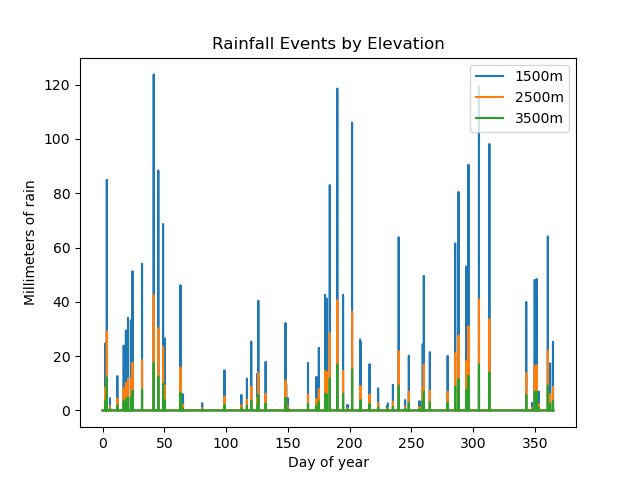
\includegraphics[width=0.67\textwidth]{rainoneyear.png}
    \caption{One Year of Simulated Rainfall Events}
    \label{fig:my_label}
\end{figure}

Generated rainfall data, displayed in Figure 1, exhibits the expected Poisson- and exponentially-distributed properties. When compared to the soil moisture results in Figure 2, a clear correlation can be seen: soil moisture rises following significant rainfall events, and exhibits exponential decay in periods of low rainfall.

\begin{figure}[hp]
    \centering
    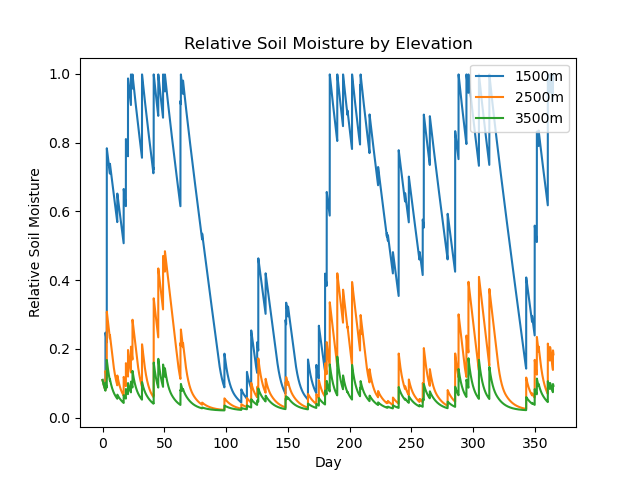
\includegraphics[width=0.67\textwidth]{soilmoistureoneyear.png}
    \caption{One Year of Simulated Soil Moisture by Elevation}
    \label{fig:my_label}
\end{figure}

As expected, soil moisture values are the highest at low elevations, which receive significantly more rainfall. Following periods of very high rainfall, the capacity constraint is also exhibited: soil moisture never exceeds 1, the maximum proportion able to be held of soil with a given porosity.

Trends in carbon content vary significantly by pool. The humus pool is relatively stable; changes are nearly imperceptible when viewed on a 20-year scale, and again very slight when observed over 500 years as shown in Figure 3. By elevation, carbon accumulation in the humus is the highest of the simulations, due to decreased decomposition as a result of lower average soil moisture.

\begin{figure}[hp]
    \centering
    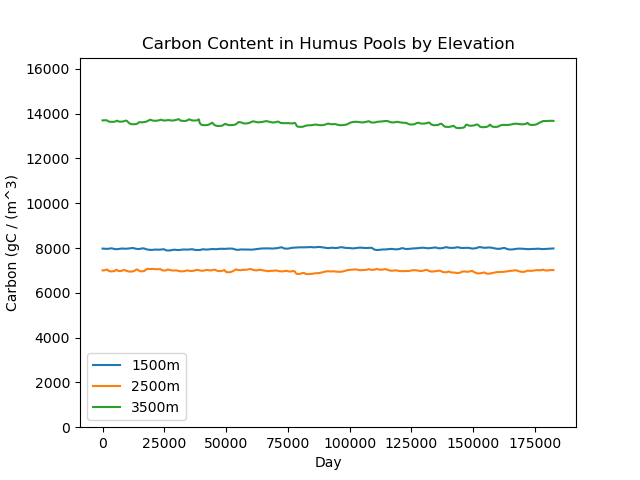
\includegraphics[width=0.67\textwidth]{humus500years.png}
    \caption{Humus Carbon Content over 500 Years}
    \label{fig:my_label}
\end{figure}

The biomass pool, on the other hand, exhibits the largest magnitude of swings in carbon content. As shown in Figure 4, biomass carbon appears to follow a cyclical trend; the values at higher elevations tend to spike together, while the value at the lowest elevation has the opposite pattern. The period for this cycle appears to be about 10 years.

\begin{figure}[hp]
    \centering
    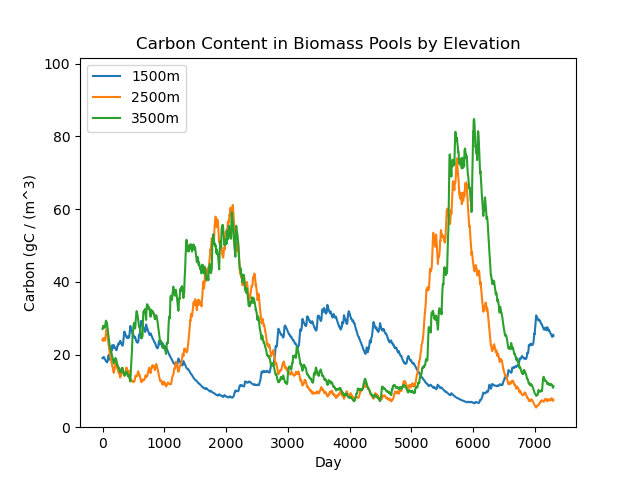
\includegraphics[width=0.67\textwidth]{biomass20years.png}
    \caption{Biomass Carbon Content over 20 Years}
    \label{fig:my_label}
\end{figure}

Finally, the litter pool exhibits a similar cyclical pattern to the humus pool, albeit on a scale which is smoother and smaller in magnitude. This is shown on a 20-year scale in Figure 5, and a 500-year scale in Figure 6. One significant pattern to note is that the carbon content in the litter pool increases at nearly the litterfall rate when the biomass carbon is low, and then sharply declines when biomass carbon increases. Thus, the approximately 10-year period of these cycles is consistent between pools. 

\begin{figure}[hp]
    \centering
    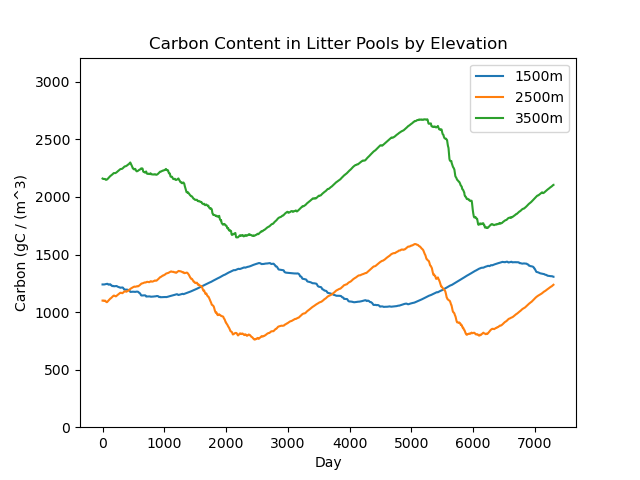
\includegraphics[width=0.67\textwidth]{litter20years.png}
    \caption{Litter Carbon Content over 20 Years}
    \label{fig:my_label}
\end{figure}

Numerical averages and standard deviations for the carbon content in each pool over 500 years, by elevation, are shown in Table 3.

\begin{table}[hp]
\begin{center}
\begin{tabular}{ c c c c c }
Pool & 1500m & 2500m & 3500m & Units \\
\hline 
Litter & $1245.0 \pm 125.1$ & $1095.6 \pm 125.3$ & $2160.6 \pm 323.3$ & gC/m\textsuperscript{2} \\
Humus & $7986.2 \pm 29.2$ & $6972.2 \pm 48.4$ & $13537.2 \pm 83.7$ & gC/m\textsuperscript{2} \\
Biomass & $19.3 \pm 7.0$ & $23.6 \pm 8.5$ & $26.8 \pm 16.6$ & gC/m\textsuperscript{2}

\end{tabular}
\end{center}
\caption{\label{tab:table-name}Averages and Standard Deviations of Carbon Content in Pools}
\end{table}

\section{Discussion}
This model is relevant to present-day concerns regarding how ecosystems will respond to moisture-related changes induced by climate change. Given that prolonged and more frequent drought events have been occurring in many ecosystems across the world, this is an important dynamic to be able to model. \cite{oconnell_drought_2018,staal_hysteresis_2020} As low moisture causes both water and nutrient stress in plants, we need to be able to predict the resilience of ecosystems to these changes in order to predict how our natural areas will be impacted with worsening climate change. \cite{cusack_seasonal_2019} In the Amazon for example, plant responses to drought have been implicated in contributing to hydrological feedback mechanisms that worsen drought scenarios, to the point where many scientists believe that the Amazon has reached a hydrological tipping point where it may flip to a drier temperate forest or savanna ecosystem. \cite{oconnell_drought_2018,staal_hysteresis_2020} This is an extreme example, but this model, and those similar to it, can help predict similar patterns across the natural areas of the world.

The results of our model show that accumulation in organic carbon pools is much higher in the lower rainfall area, which is consistent with the decrease in decomposition that we expect with low moisture. This result does not exactly reflect the reality of the Mauna Kea area, as vascular plants do not grow at that rainfall level. \cite{bateman_quantitative_2019} However, if each area had the same or similar vegetation this result would be fairly accurate. In arid or semi-arid ecosystems, for example, carbon and other nutrients are mostly located in soil organic pools. \cite{cairney_ericoid_2003} One result that is not entirely consistent with observed patterns is the low amount of carbon in the microbial biomass pool in the high rainfall area relative to the lower rainfall areas. A possible explanation for this is the parabolic relationship between decomposition and soil moisture that we applied in this model. \cite{cusack_seasonal_2019,porporato_hydrologic_2003} In many systems, high moisture levels suppress decomposition by creating anaerobic conditions for microbes, while low moisture levels lead to microbial desiccation. \cite{schimel_life_2018} Though Mauna Kea’s rainfall is not extremely high, the moisture level at low elevations is relatively much higher than that of higher elevations.

Our model appears to accurately represent the short-term influences of soil moisture on carbon cycling. Our results for short-term runs are consistent with patterns shown by Porporato et. al’s model, though nuanced responses can be expected with changes in initial parameters. \cite{porporato_hydrologic_2003,dodorico_hydrologic_2003}

This model is a simplified version of the dynamics between nutrient cycling and moisture changes, so there are many possible sources of error. In terms of rainfall, we ignore seasonality of rainfall, instead having consistent random rainfall spikes throughout the year. This works in our application of the model to the windward side of Mauna Kea, as rainfall is fairly constant throughout the year. \cite{giambelluca_online_2013} However, if this model were to be applied to seasonal systems this would need to be adjusted. Also, as addressed in the parameter section, some values that were used in applying this model to the Mauna Kea gradient were based on values from the companion paper to Porporato et. al. \cite{dodorico_hydrologic_2003} Their parameter values were largely gathered through measurements in the field, which would be necessary to replicate in order to apply our model to Mauna Kea as accurately as possible.



\bibliography{citations}{}
\bibliographystyle{plain}

\begin{figure}[p]
    \centering
    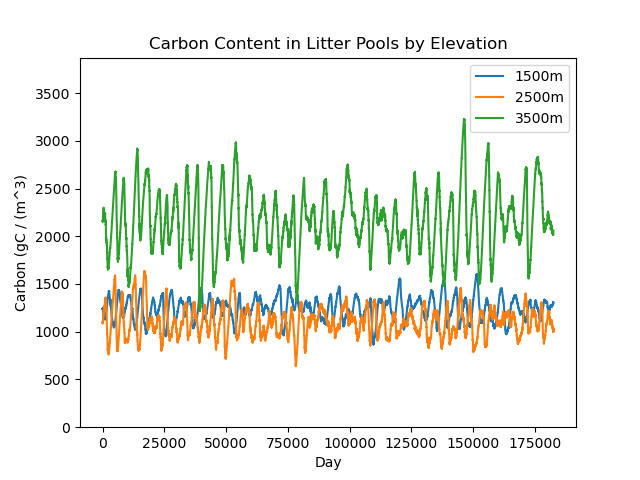
\includegraphics[width=0.67\textwidth]{litter500years.png}
    \caption{Litter Carbon Content over 500 Years}
    \label{fig:my_label}
\end{figure}

\begin{figure}[p]
    \centering
    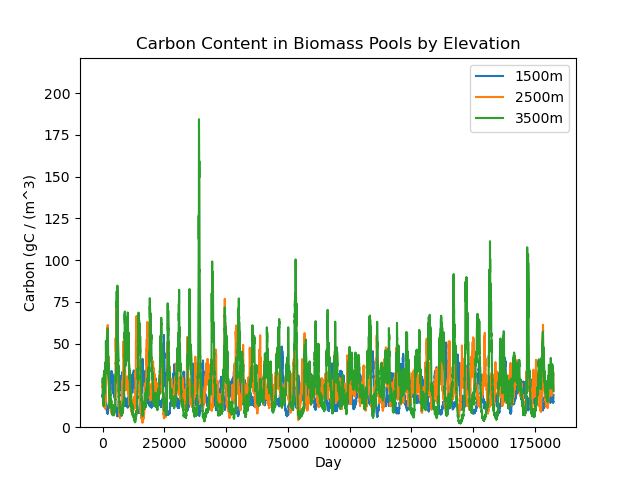
\includegraphics[width=0.67\textwidth]{biomass500years.png}
    \caption{Biomass Carbon Content over 500 Years}
    \label{fig:my_label}
\end{figure}

\end{document}
